\documentclass[DIV=14,titlepage=false]{scrreprt}
%%%%%%%%%%%%%%%%%%%%%%%%%%%%%%%%%%%%%%%%%%%%%%%%%%%%%%%%%%%%%%%%%%%%%%%%%%%%%%%
%                                Basic Packages                               %
%%%%%%%%%%%%%%%%%%%%%%%%%%%%%%%%%%%%%%%%%%%%%%%%%%%%%%%%%%%%%%%%%%%%%%%%%%%%%%%
% Gives us multiple colors.
\usepackage[usenames,dvipsnames,pdftex]{xcolor}
% Lets us style link colors.
\usepackage{hyperref}
% Lets us import images and graphics.
\usepackage{graphicx}
% Lets us use figures in floating environments.
\usepackage{float}
% Lets us create multiple columns.
\usepackage{multicol}
% Gives us better math syntax.
\usepackage{amsmath,amsfonts,mathtools,amsthm,amssymb}
% Lets us strikethrough text.
\usepackage{cancel}
% Lets us edit the caption of a figure.
\usepackage{caption}
% Lets us import pdf directly in our tex code.
\usepackage{pdfpages}
% Lets us do algorithm stuff.
\usepackage[ruled,vlined,linesnumbered]{algorithm2e}
% Gets rid of some errors.
\usepackage{scrhack}
\def\class{article}
\usepackage{geometry}
\geometry{margin=0.9in}
%%%%%%%%%%%%%%%%%%%%%%%%%%%%%%%%%%%%%%%%%%%%%%%%%%%%%%%%%%%%%%%%%%%%%%%%%%%%%%%
%                                Basic Settings                               %
%%%%%%%%%%%%%%%%%%%%%%%%%%%%%%%%%%%%%%%%%%%%%%%%%%%%%%%%%%%%%%%%%%%%%%%%%%%%%%%

%%%%%%%%%%%%%
%  Symbols  %
%%%%%%%%%%%%%

\let\implies\Rightarrow
\let\impliedby\Leftarrow
\let\iff\Leftrightarrow
\let\epsilon\varepsilon

%%%%%%%%%%%%
%  Tables  %
%%%%%%%%%%%%

\setlength{\tabcolsep}{5pt}
\renewcommand\arraystretch{1.5}

%%%%%%%%%%%%%%%%%%%%%%%
%  Center Title Page  %
%%%%%%%%%%%%%%%%%%%%%%%

\usepackage{titling}
\renewcommand\maketitlehooka{\null\mbox{}\vfill}
\renewcommand\maketitlehookd{\vfill\null}

%%%%%%%%%%%%%%%%%%%%%%%%%%%%%%%%%%%%%%%%%%%%%%%%%%%%%%%
%  Create a grey background in the middle of the PDF  %
%%%%%%%%%%%%%%%%%%%%%%%%%%%%%%%%%%%%%%%%%%%%%%%%%%%%%%%

\usepackage{eso-pic}
\newcommand\definegraybackground{
  \definecolor{reallylightgray}{HTML}{FAFAFA}
  \AddToShipoutPicture{
    \ifthenelse{\isodd{\thepage}}{
      \AtPageLowerLeft{
        \put(\LenToUnit{\dimexpr\paperwidth-222pt},0){
          \color{reallylightgray}\rule{222pt}{297mm}
        }
      }
    }
    {
      \AtPageLowerLeft{
        \color{reallylightgray}\rule{222pt}{297mm}
      }
    }
  }
}

%%%%%%%%%%%%%%%%%%%%%%%%
%  Modify Links Color  %
%%%%%%%%%%%%%%%%%%%%%%%%

\hypersetup{
  % Enable highlighting links.
  colorlinks,
  % Change the color of links to blue.
  linkcolor={black},
  % Change the color of citations to black.
  citecolor={black},
  % Change the color of url's to blue with some black.
  urlcolor=blue
}

%%%%%%%%%%%%%%%%%%
% Fix WrapFigure %
%%%%%%%%%%%%%%%%%%

\newcommand{\wrapfill}{\par\ifnum\value{WF@wrappedlines}>0
    \parskip=0pt
    \addtocounter{WF@wrappedlines}{-1}%
    \null\vspace{\arabic{WF@wrappedlines}\baselineskip}%
    \WFclear
\fi}

%%%%%%%%%%%%%%%%%
% Multi Columns %
%%%%%%%%%%%%%%%%%

\let\multicolmulticols\multicols
\let\endmulticolmulticols\endmulticols

\RenewDocumentEnvironment{multicols}{mO{}}
{%
  \ifnum#1=1
    #2%
  \else % More than 1 column
    \multicolmulticols{#1}[#2]
  \fi
}
{%
  \ifnum#1=1
\else % More than 1 column
  \endmulticolmulticols
\fi
}

\newlength{\thickarrayrulewidth}
\setlength{\thickarrayrulewidth}{5\arrayrulewidth}

%%%%%%%%%%%%%%%%%%%%
%  Import Figures  %
%%%%%%%%%%%%%%%%%%%%

\usepackage{import}
\pdfminorversion=7

% EXAMPLE:
% 1. \incfig{limit-graph}
% 2. \incfig[0.4]{limit-graph}
% Parameters:
% 1. The figure name. It should be located in figures/NAME.tex_pdf.
% 2. (Optional) The width of the figure. Example: 0.5, 0.35.
\newcommand\incfig[2][1]{%
  \def\svgwidth{#1\columnwidth}
  \import{./figures/}{#2.pdf_tex}
}

\begingroup\expandafter\expandafter\expandafter\endgroup
\expandafter\ifx\csname pdfsuppresswarningpagegroup\endcsname\relax
\else
  \pdfsuppresswarningpagegroup=1\relax
\fi

%%%%%%%%%%%%%
%  Correct  %
%%%%%%%%%%%%%

% EXAMPLE:
% 1. \correct{INCORRECT}{CORRECT}
% Parameters:
% 1. The incorrect statement.
% 2. The correct statement.
\definecolor{correct}{HTML}{009900}
\newcommand\correct[2]{{\color{red}{#1 }}\ensuremath{\to}{\color{correct}{ #2}}}



\newcommand{\R}{\mathbb{R}}
\newcommand{\Z}{\mathbb{Z}}
\newcommand{\E}{\mathbb{E}}
\newcommand{\B}{\ensuremath{\mathcal{B}}}
\newcommand{\X}{\ensuremath{\mathcal{X}}}
\newcommand{\Y}{\ensuremath{\mathcal{Y}}}
\newcommand{\mA}{\ensuremath{\mathbf{A}}}
\newcommand{\mB}{\ensuremath{\mathbf{B}}}
\newcommand{\mC}{\ensuremath{\mathbf{C}}}
\newcommand{\mD}{\ensuremath{\mathbf{D}}}
\newcommand{\mX}{\ensuremath{\mathbf{X}}}
\newcommand{\mY}{\ensuremath{\mathbf{Y}}}
\newcommand{\mx}{\ensuremath{\mathbf{x}}}
\newcommand{\my}{\ensuremath{\mathbf{y}}}
\newcommand{\mI}{\ensuremath{\mathbf{I}}}
\newcommand{\mi}{\ensuremath{\mathbf{\iota}}}
\newcommand{\mmu}{\ensuremath{\mathbf{\mu}}}
\newcommand{\mc}{\ensuremath{\mathbf{c}}}
\newcommand{\mSigma}{\ensuremath{\mathbf{\Sigma}}}
\newcommand{\mzero}{\ensuremath{\mathbf{0}}}
\newcommand{\independent}{\perp\!\!\!\!\perp} 
\setlength{\parindent}{0pt}
%%%%%%%%%%%%%%%%%%%%%%%%%%%%%%%%%%%%%%%%%%%%%%%%%%%%%%%%%%%%%%%%%%%%%%%%%%%%%%%
%                                 Environments                                %
%%%%%%%%%%%%%%%%%%%%%%%%%%%%%%%%%%%%%%%%%%%%%%%%%%%%%%%%%%%%%%%%%%%%%%%%%%%%%%%

\usepackage{varwidth}
\usepackage{thmtools}
\usepackage[most,many,breakable]{tcolorbox}

\tcbuselibrary{theorems,skins,hooks}
\usetikzlibrary{arrows,calc,shadows.blur}

%%%%%%%%%%%%%%%%%%%
%  Define Colors  %
%%%%%%%%%%%%%%%%%%%

\definecolor{myblue}{RGB}{45, 111, 177}
\definecolor{mygreen}{RGB}{56, 140, 70}
\definecolor{myred}{RGB}{199, 68, 64}
\definecolor{mypurple}{RGB}{197, 92, 212}

\definecolor{definition}{HTML}{228b22}
\definecolor{theorem}{HTML}{00007B}
\definecolor{example}{HTML}{2A7F7F}
\definecolor{definition}{HTML}{228b22}
\definecolor{prop}{HTML}{191971}
\definecolor{lemma}{HTML}{983b0f}
\definecolor{exercise}{HTML}{88D6D1}

\colorlet{definition}{mygreen!85!black}
\colorlet{claim}{mygreen!85!black}
\colorlet{corollary}{mypurple!85!black}
\colorlet{proof}{theorem}

%%%%%%%%%%%%%%%%%%%%%%
%  Helpful Commands  %
%%%%%%%%%%%%%%%%%%%%%%

% EXAMPLE:
% 1. \createnewtheoremstyle{thmdefinitionbox}{}{}
% 2. \createnewtheoremstyle{thmtheorembox}{}{}
% 3. \createnewtheoremstyle{thmproofbox}{qed=\qedsymbol}{
%       rightline=false, topline=false, bottomline=false
%    }
% Parameters:
% 1. Theorem name.
% 2. Any extra parameters to pass directly to declaretheoremstyle.
% 3. Any extra parameters to pass directly to mdframed.
\newcommand\createnewtheoremstyle[3]{
  \declaretheoremstyle[
  headfont=\bfseries\sffamily, bodyfont=\normalfont, #2,
  mdframed={
    #3,
  },
  ]{#1}
}

% EXAMPLE:
% 1. \createnewcoloredtheoremstyle{thmdefinitionbox}{definition}{}{}
% 2. \createnewcoloredtheoremstyle{thmexamplebox}{example}{}{
%       rightline=true, leftline=true, topline=true, bottomline=true
%     }
% 3. \createnewcoloredtheoremstyle{thmproofbox}{proof}{qed=\qedsymbol}{backgroundcolor=white}
% Parameters:
% 1. Theorem name.
% 2. Color of theorem.
% 3. Any extra parameters to pass directly to declaretheoremstyle.
% 4. Any extra parameters to pass directly to mdframed.
\newcommand\createnewcoloredtheoremstyle[4]{
  \declaretheoremstyle[
  headfont=\bfseries\sffamily\color{#2}, bodyfont=\normalfont, #3,
  mdframed={
    linewidth=2pt,
    rightline=false, leftline=true, topline=false, bottomline=false,
    linecolor=#2, backgroundcolor=#2!5, #4,
  },
  ]{#1}
}

%%%%%%%%%%%%%%%%%%%%%%%%%%%%%%%%%%%
%  Create the Environment Styles  %
%%%%%%%%%%%%%%%%%%%%%%%%%%%%%%%%%%%

\makeatletter
\@ifclasswith\class{nocolor}{
  % Environments without color.

  \createnewtheoremstyle{thmdefinitionbox}{}{}
  \createnewtheoremstyle{thmtheorembox}{}{}
  \createnewtheoremstyle{thmexamplebox}{}{}
  \createnewtheoremstyle{thmclaimbox}{}{}
  \createnewtheoremstyle{thmcorollarybox}{}{}
  \createnewtheoremstyle{thmpropbox}{}{}
  \createnewtheoremstyle{thmlemmabox}{}{}
  \createnewtheoremstyle{thmexercisebox}{}{}
  \createnewtheoremstyle{thmdefinitionbox}{}{}
  \createnewtheoremstyle{thmquestionbox}{}{}
  \createnewtheoremstyle{thmsolutionbox}{}{}

  \createnewtheoremstyle{thmproofbox}{qed=\qedsymbol}{}
  \createnewtheoremstyle{thmexplanationbox}{}{}
}{
  % Environments with color.

  \createnewcoloredtheoremstyle{thmdefinitionbox}{definition}{}{}
  \createnewcoloredtheoremstyle{thmtheorembox}{theorem}{}{}
  \createnewcoloredtheoremstyle{thmexamplebox}{example}{}{
    rightline=true, leftline=true, topline=true, bottomline=true
  }
  \createnewcoloredtheoremstyle{thmclaimbox}{claim}{}{}
  \createnewcoloredtheoremstyle{thmcorollarybox}{corollary}{}{}
  \createnewcoloredtheoremstyle{thmpropbox}{prop}{}{}
  \createnewcoloredtheoremstyle{thmlemmabox}{lemma}{}{}
  \createnewcoloredtheoremstyle{thmexercisebox}{exercise}{}{}

  \createnewcoloredtheoremstyle{thmproofbox}{proof}{qed=\qedsymbol}{backgroundcolor=white}
  \createnewcoloredtheoremstyle{thmexplanationbox}{example}{qed=\qedsymbol}{backgroundcolor=white}
}
\makeatother

%%%%%%%%%%%%%%%%%%%%%%%%%%%%%
%  Create the Environments  %
%%%%%%%%%%%%%%%%%%%%%%%%%%%%%

\declaretheorem[numberwithin=section, style=thmtheorembox,     name=Theorem]{theorem}
\declaretheorem[numbered=no,          style=thmexamplebox,     name=Example]{example}
\declaretheorem[numberwithin=section, style=thmclaimbox,       name=Claim]{claim}
\declaretheorem[numberwithin=section, style=thmcorollarybox,   name=Corollary]{corollary}
\declaretheorem[numberwithin=section, style=thmpropbox,        name=Proposition]{prop}
\declaretheorem[numberwithin=section, style=thmlemmabox,       name=Lemma]{lemma}
\declaretheorem[numberwithin=section, style=thmexercisebox,    name=Exercise]{exercise}
\declaretheorem[numbered=no,          style=thmproofbox,       name=Proof]{replacementproof}
\declaretheorem[numbered=no,          style=thmexplanationbox, name=Proof]{expl}

\makeatletter
\@ifclasswith\class{nocolor}{
  % Environments without color.

  \newtheorem*{note}{Note}

  \declaretheorem[numberwithin=section, style=thmdefinitionbox, name=Definition]{definition}
  \declaretheorem[numberwithin=section, style=thmquestionbox,   name=Question]{question}
  \declaretheorem[numberwithin=section, style=thmsolutionbox,   name=Solution]{solution}
}{
  % Environments with color.

  \newtcbtheorem[number within=section]{Definition}{Definition}{
    enhanced,
    before skip=2mm,
    after skip=2mm,
    colback=red!5,
    colframe=red!80!black,
    colbacktitle=red!75!black,
    boxrule=0.5mm,
    attach boxed title to top left={
      xshift=1cm,
      yshift*=1mm-\tcboxedtitleheight
    },
    varwidth boxed title*=-3cm,
    boxed title style={
      interior engine=empty,
      frame code={
        \path[fill=tcbcolback]
        ([yshift=-1mm,xshift=-1mm]frame.north west)
        arc[start angle=0,end angle=180,radius=1mm]
        ([yshift=-1mm,xshift=1mm]frame.north east)
        arc[start angle=180,end angle=0,radius=1mm];
        \path[left color=tcbcolback!60!black,right color=tcbcolback!60!black,
        middle color=tcbcolback!80!black]
        ([xshift=-2mm]frame.north west) -- ([xshift=2mm]frame.north east)
        [rounded corners=1mm]-- ([xshift=1mm,yshift=-1mm]frame.north east)
        -- (frame.south east) -- (frame.south west)
        -- ([xshift=-1mm,yshift=-1mm]frame.north west)
        [sharp corners]-- cycle;
      },
    },
    fonttitle=\bfseries,
    title={#2},
    #1
  }{def}

  \NewDocumentEnvironment{definition}{O{}O{}}
    {\begin{Definition}{#1}{#2}}{\end{Definition}}

  \newtcolorbox{note}[1][]{%
    enhanced jigsaw,
    colback=gray!20!white,%
    colframe=gray!80!black,
    size=small,
    boxrule=1pt,
    title=\textbf{Note:-},
    halign title=flush center,
    coltitle=black,
    breakable,
    drop shadow=black!50!white,
    attach boxed title to top left={xshift=1cm,yshift=-\tcboxedtitleheight/2,yshifttext=-\tcboxedtitleheight/2},
    minipage boxed title=1.5cm,
    boxed title style={%
      colback=white,
      size=fbox,
      boxrule=1pt,
      boxsep=2pt,
      underlay={%
        \coordinate (dotA) at ($(interior.west) + (-0.5pt,0)$);
        \coordinate (dotB) at ($(interior.east) + (0.5pt,0)$);
        \begin{scope}
          \clip (interior.north west) rectangle ([xshift=3ex]interior.east);
          \filldraw [white, blur shadow={shadow opacity=60, shadow yshift=-.75ex}, rounded corners=2pt] (interior.north west) rectangle (interior.south east);
        \end{scope}
        \begin{scope}[gray!80!black]
          \fill (dotA) circle (2pt);
          \fill (dotB) circle (2pt);
        \end{scope}
      },
    },
    #1,
  }

  \newtcbtheorem{Question}{Question}{enhanced,
    breakable,
    colback=white,
    colframe=myblue!80!black,
    attach boxed title to top left={yshift*=-\tcboxedtitleheight},
    fonttitle=\bfseries,
    title=\textbf{Question:-},
    boxed title size=title,
    boxed title style={%
      sharp corners,
      rounded corners=northwest,
      colback=tcbcolframe,
      boxrule=0pt,
    },
    underlay boxed title={%
      \path[fill=tcbcolframe] (title.south west)--(title.south east)
      to[out=0, in=180] ([xshift=5mm]title.east)--
      (title.center-|frame.east)
      [rounded corners=\kvtcb@arc] |-
      (frame.north) -| cycle;
    },
    #1
  }{def}

  \NewDocumentEnvironment{question}{O{}O{}}
  {\begin{Question}{#1}{#2}}{\end{Question}}

  \newtcolorbox{Solution}{enhanced,
    breakable,
    colback=white,
    colframe=mygreen!80!black,
    attach boxed title to top left={yshift*=-\tcboxedtitleheight},
    title=\textbf{Solution:-},
    boxed title size=title,
    boxed title style={%
      sharp corners,
      rounded corners=northwest,
      colback=tcbcolframe,
      boxrule=0pt,
    },
    underlay boxed title={%
      \path[fill=tcbcolframe] (title.south west)--(title.south east)
      to[out=0, in=180] ([xshift=5mm]title.east)--
      (title.center-|frame.east)
      [rounded corners=\kvtcb@arc] |-
      (frame.north) -| cycle;
    },
  }

  \NewDocumentEnvironment{solution}{O{}O{}}
  {\vspace{-10pt}\begin{Solution}{#1}{#2}}{\end{Solution}}
}
\makeatother

%%%%%%%%%%%%%%%%%%%%%%%%%%%%
%  Edit Proof Environment  %
%%%%%%%%%%%%%%%%%%%%%%%%%%%%

\renewenvironment{proof}[1][\proofname]{\vspace{-10pt}\begin{replacementproof}}{\end{replacementproof}}
\newenvironment{explanation}[1][\proofname]{\vspace{-10pt}\begin{expl}}{\end{expl}}

\theoremstyle{definition}

\newtheorem*{notation}{Notation}
\newtheorem*{previouslyseen}{As previously seen}
\newtheorem*{problem}{Problem}
\newtheorem*{observe}{Observe}
\newtheorem*{property}{Property}
\newtheorem*{intuition}{Intuition}

\setuptoc{toc}{leveldown}

\begin{document}
\setcounter{chapter}{8}
\pagenumbering{gobble}
\vspace{-10pt}


\chapter{Functional CLT. Fixed-b asymptotics.}

\section{Fixed bandwidth approach}
The choice of truncation lag G in the Newey-West method is arbitrary. There are many ways of choosing this lag optimally, see Andrews (1991) for an example. \\
Kiefer, Vogelsang and Bunzel (2000) show that the accuracy of the tests based on the Newey-West variance estimator may be quite poor in finite samples, specifically tests over-reject the null (the estimated variance is 'too small'). They proposed an alternative where G is chosen such that $b\equiv \frac{G+1}{T}\to 0$ as $T\to \infty$. $b$ is known as the bandwidth, and is kept fixed. For example, when G+1=T, $b$ is fixed at 1. Under this approach $\hat V$ converges to a limiting random matrix that is proportional to $V$. The distribution of HAC robust tests based on $\hat V$ don't depend on the model's parameters (i.e. the distribution is pivotal), and can be tabulated.

\begin{definition}[Long-run variance]
    Sum of all the variances and covariances of a process, i.e. Var($\sum_{t=1}^T \epsilon_t$).
\end{definition}


    Consider the simple regression on only a constant term \[ Y_t = \beta + \epsilon_t.\] The OLS estimator of $\beta$ is $\hat \beta_{OLS} = \bar Y$, and under serial correlation:
    \[
    Var(\hat \beta_{OLS})=\frac{1}{T} V_T = \frac{1}{T} \left(\E \epsilon_t^2 + \sum_{\ell=1}^{T-1}\frac{T-\ell}{T} 2\E(\epsilon_t \epsilon_{t-\ell}) \right) \not = \frac{1}{T} Var(\epsilon_t)
    \]
    where the first equality follows from the previous lecture. As $T\to \infty$, the variance of the OLS estimator converges to the long-run variance of $\epsilon_t$. \\
    \textbf{Newey-West}
    \[
    \hat V_{NW} = \frac{1}{T} \sum_{t=1}^{T} \hat \epsilon_t^2 + \sum_{\ell=1}^{G}\frac{G+1-\ell}{G+1} \frac{2}{T} \sum_{t=1+\ell}^{T} \hat \epsilon_t \hat \epsilon_{t-\ell}\]
    \textbf{KVB}\\
    KVB obtains an inconsistent estimator of $V_T$ with $G=T-1$:
    \[
        \hat{V}_{KVB} = \frac{1}{T} \sum_{t=1}^{T} \hat \epsilon_t^2 + \sum_{\ell=1}^{T-1}\frac{T-\ell}{T} \frac{2}{T} \sum_{t=1+\ell}^{T} \hat \epsilon_t \hat \epsilon_{t-\ell}
    \]
    Here $\hat \epsilon_t= Y_t - \bar Y$.

    We can show that $\hat V_{KVB}$ is positive semi-definite as follows:
    \begin{align*}
        \hat V_{KVB} &= \frac{1}{T} \sum_{t=1}^{T} \hat \epsilon_t^2 + \sum_{\ell=1}^{T-1}\frac{T-\ell}{T} \frac{2}{T} \sum_{t=1+\ell}^{T} \hat \epsilon_t \hat \epsilon_{t-\ell}\\
        &= \frac{1}{T} \mathbf{1'}\left(\frac{1}{T} \sum_{t=1+|i-j|}^{T} \hat \epsilon_t \hat \epsilon_{t-|i-j|}\right)\mathbf{1}\quad \text{where 1 is a T-vector of ones}\\
        &= \frac{1}{T^2} \mathbf{1'}ZZ'\mathbf{1} \\
        \text{where} \underbrace{Z}_{T \times (2T-1)}&= \begin{bmatrix}
            \hat \epsilon_1 & \hat \epsilon_2 & \cdots & \hat \epsilon_T & 0 & \cdots & 0\\
            0 & \hat \epsilon_1 & \cdots & \hat \epsilon_{T-1} & \hat \epsilon_T & \cdots & 0\\
            \vdots & \vdots & \ddots & \vdots & \vdots & \ddots & \vdots\\
            0 & 0 & \cdots & \hat \epsilon_1 & \hat \epsilon_2 & \cdots & \hat \epsilon_T
        \end{bmatrix}
    \end{align*}
    Thus $\hat V_{KVB}$ is positive semi-definite. Further, since $\sum_{t=1}^{T}\hat\epsilon_t=0$ (property of OLS residuals) the sum of elements in the T-th column is zero. Moreover, the sum of elements in the $T+i$-th column gives:
    \begin{align*}
        \sum_{t=i+1}^{T} \hat \epsilon_t &= \sum_{t=0}^{T} \hat \epsilon_t - \sum_{t=0}^{i} \hat \epsilon_t\\
        &= 0 - \sum_{t=0}^{i} \hat \epsilon_t
    \end{align*}
    Thus,
    \[
        \mathbf{1'}Z = \left( \sum_{i=1}^{1} \hat \epsilon_i, \sum_{i=1}^{2} \hat \epsilon_i, \cdots, \sum_{i=1}^{T-1}, 0, - \sum_{i=1}^{1} \hat \epsilon_i, - \sum _{i=1}^{2} \hat \epsilon_i, \cdots, - \sum_{i=1}^{T-1} \hat \epsilon_i \right)
    \]
    Hence,
    \begin{align*}
        \hat V_{KVB} &= \frac{1}{T^2} \mathbf{1'}ZZ'\mathbf{1}\\
        &= \frac{1}{T^2} 
        \begin{bmatrix}
            \sum_{i=1}^{1} \hat \epsilon_i & \cdots & \sum_{i=1}^{T-1} \hat \epsilon_i & 0 & - \sum_{i=1}^{1} \hat \epsilon_i & \cdots & - \sum_{i=1}^{T-1} \hat \epsilon_i
        \end{bmatrix}
        \begin{bmatrix}
            \sum_{i=1}^{1} \hat \epsilon_i \\
            \vdots\\
            \sum_{i=1}^{T-1} \hat \epsilon_i \\
            0\\
            - \sum_{i=1}^{1} \hat \epsilon_i\\
            \vdots\\
            - \sum_{i=1}^{T-1} \hat \epsilon_i
        \end{bmatrix}\\
        &= \frac{1}{T^2} \left( \left(\sum_{i=1}^{1} \hat \epsilon_i\right)^2 +  \cdots + \left(\sum_{i=1}^{T-1} \hat \epsilon_i\right)^2 + 0 + \left(- \sum_{i=1}^{1} \hat \epsilon_i\right)^2 + \cdots + \left(- \sum_{i=1}^{T-1} \hat \epsilon_i\right)^2 \right)\\
        &= \frac{2}{T^2} \sum_{s=1}^{T-1} \left(\sum_{i=1}^{s}\hat \epsilon_i\right)^2\\
        &= \frac{2}{T} \sum_{s=1}^{T-1} \left(\frac{1}{\sqrt{T}}\sum_{i=1}^{s}\hat \epsilon_i\right)^2\\
    \end{align*}
    We know that $\hat \epsilon_t = Y_t - \bar Y=\beta + \epsilon_t - (\beta +\bar \epsilon) = \epsilon_t - \bar \epsilon$.
    \begin{align*}
        \hat V_{KVB} &= \frac{2}{T} \sum_{s=1}^{T-1} \left(\frac{1}{\sqrt{T}}\sum_{i=1}^{s}\hat \epsilon_i\right)^2\\
        &= \frac{2}{T} \sum_{s=1}^{T-1} \left(\frac{1}{\sqrt{T}}\sum_{i=1}^{s}(\epsilon_i - \bar \epsilon)\right)^2\\
        &= \frac{2}{T} \sum_{s=1}^{T-1} \left(\frac{1}{\sqrt{T}}\sum_{i=1}^{s}\epsilon_i -\frac{s}{\sqrt{T}} \bar \epsilon\right)^2\\
        &= \frac{2}{T} \sum_{s=1}^{T-1} \left(\frac{1}{\sqrt{T}}\sum_{i=1}^{s}\epsilon_i -\frac{s}{T}\frac{1}{\sqrt{T}} \sum_{i=1}^{T}\epsilon_i\right)^2\\
    \end{align*}
\section{Functional CLT}
We first introduce the concept of Brownian motion (or the Wiener process). 

\begin{definition}[Brownian motion]
    The standard Brownian motion $W(\lambda), \lambda \in [0,1]$ is a continuous time stochastic process such that $W(\lambda_1), \dots, W(\lambda_k)$ are jointly normally distributed for any $k \in [0,1]$ for fixed $\lambda_1, \dots, \lambda_k$ with:
    \[ \E W(\lambda_i) = 0, \quad Cov(W(\lambda_i), W(\lambda_j)) = \min(\lambda_i, \lambda_j) \quad \forall i,j \in [0,1]\]
\end{definition}
This is to say, it is a set of random variables indexed by $\lambda$, or alternatively a random function in C[0,1] the space of continuous functions on [0,1]. Further any interval of indices within $W(\lambda)$ is jointly normal.\\
\textbf{Properties}
\begin{itemize}
    \item Var($W(\lambda_i)$) = $\lambda_i$
    \subitem Var($W(\lambda_i)$) = Cov($W(\lambda_i), W(\lambda_i)$) = min($\lambda_i, \lambda_i$) = $\lambda_i$
    \item $W(0) = 0$
    \subitem $\E W(0) = 0$ and Var($W(0)$) = 0
    \item $W(\lambda)$ has independent increments, for every $0\leq \lambda_1 < \lambda_2 < \dots < \lambda_k \leq 1$ the random variables $W(\lambda_1), W(\lambda_2) - W(\lambda_1), \dots, W(\lambda_k) - W(\lambda_{k-1})$ are independent.
    \item $W(\lambda)$ has gaussian increments, $W(\lambda_{i+u}) - W(\lambda_i) \sim N(0, u)$
    \item $W(\lambda)$ is nowhere differentiable
\end{itemize}
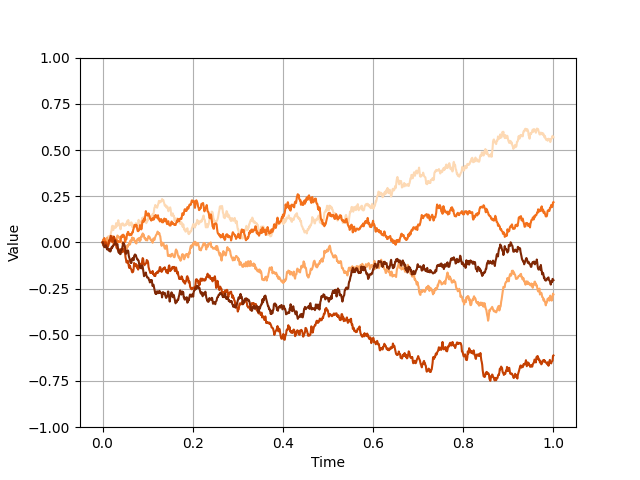
\includegraphics[width=\textwidth]{./Images/BrownianMotion.png}

The functional central limit theorem (FCLT) is a generalisation of the conventional CLT to function-valued random variables. To understand this we first generalise the standard notions of consistency and convergence in distribution to the space $C[0,1]$. We define the distance between two functions using the sup-norm:
\[
    d(f,g) = \sup_{x \in [0,1]} |f(x) - g(x)|
\]
This represents the maximum distance between the two functions.\\
\begin{definition}[Convergence in probability]
    A random element $\xi_T \in C[0,1]$ converges in probability to $f$ (that i, $\xi_T \xrightarrow{p} f$) if Pr$[d(\xi_T, f) > \delta] \to 0$ for all $\delta > 0$.
\end{definition}

\begin{definition}[Convergence in distribution]
Let \{$\xi_T$\} be a sequence of random elements in $C[0,1]$ and let $F$ be a distribution function on $C[0,1]$, with induced probability measure $\pi_T$. Then $\pi_T$ converges weakly to $\pi$, or equivalently $\xi_T \xrightarrow{d} \xi$ where $\xi$ has probability measure $\pi$, if and only if $\int f d \pi_T \to f d \pi$ for all bounded continuous functions f: $C[0,1] \to \R$.
\end{definition}

\begin{definition}[Continuous Mapping Theorem]
    If h is a continuous functional mapping $C[0,1]$ to some metric space and $\xi_T \xrightarrow{d} \xi$ then $h(\xi_T) \xrightarrow{d} h(\xi)$.
\end{definition}
We now present some background and intuition for the functional central limit theorem.
\begin{explanation}
    Let's first consider the partial sum process, defined as $X_T(\lambda) = \frac{1}{T}\sum_{t=1}^{[T\lambda]} \zeta_t$ with $\zeta \sim WN (0,1)$. The square brackets denote the floor function (i.e. the integer part of $T \lambda$).\\
    Let's see how this partial sum looks when $T=10$ and consider $\xi_T(\lambda)$ for $\lambda = 0, 0.01, 0.1,0.2$:
    \begin{align*}
        &\lambda = 0, \quad [10 \times 0] =0: \quad X_{10}(0) = \frac{1}{10} \sum_{t=1}^{0} \zeta_t = 0\\
        &\lambda = 0.01, \quad [10 \times 0.01] =0: \quad  X_{10}(0.01) = \frac{1}{10} \sum_{t=1}^{0} \zeta_t = 0\\
        &\lambda = 0.1, \quad [10 \times 0.1] =1: \quad  X_{10}(0.1) = \frac{1}{10} \sum_{t=1}^{1} \zeta_t = \frac{\zeta_1}{10} \\
        &\lambda = 0.2, \quad [10 \times 0.2] =2: \quad  X_{10}(0.2) = \frac{1}{10} \sum_{t=1}^{2} \zeta_t = \frac{\zeta_1 + \zeta_2}{10}
    \end{align*}
    For a sequence of errors $\zeta_t$ 
    \begin{enumerate}
        \item The function $X_T(\lambda)$ is a random step function defined on [0,1].
        \item As T gets bigger the step size gets smaller, and the function becomes smoother (looking more and more like a Wiener process).
    \end{enumerate}
    Lets consider the following for any fixed $\lambda \in [0,1]$:
    \begin{align*}
        \sqrt{T} X_T(\lambda) &= \sqrt{T} \frac{1}{T} \sum_{t=1}^{[T\lambda]} \zeta_t\\
        &= \frac{1}{\sqrt{T}} \sum_{t=1}^{[T\lambda]} \zeta_t\\
        &= \frac{\sqrt{[T\lambda]}}{\sqrt{T}} \frac{1}{\sqrt{[T\lambda]}} \sum_{t=1}^{[T\lambda]} \zeta_t
    \end{align*}
    Now, as $T \to \infty$:
    \begin{align*}
        \frac{\sqrt{[T\lambda]}}{\sqrt{T}} &\to \sqrt{\lambda}\\
        \frac{1}{\sqrt{[T\lambda]}} \sum_{t=1}^{[T\lambda]} \zeta_t &\xrightarrow{d} N(0, 1) \quad \text{by the CLT}
    \end{align*}
    It follows from Slutsky's theorem that:
    \[
        \sqrt{T} X_T(\lambda) \xrightarrow{d} \sqrt{\lambda} N(0,\lambda) = W(\lambda)
    \]
    Since the above holds for any $\lambda \in [0,1]$, we might expect this holds uniformly for $\lambda \in [0,1]$. This is indeed the case, and is known as the functional central limit theorem (or Donsker's theorem for partial sums).
    \end{explanation}
The above is based on a step-function, however Alexei present a piecewise linear function where we linearly interpolate between points. This is presented below, the substantive results are the same.\\
Let $\zeta_T$, $t=1,2,...$ be zero mean i.i.d. random variables with variance 1. Let $\xi_T(\lambda)$ be the function constructed by linearly interpolating between the partial sums of $\zeta$ at the points $\lambda = (0, \frac{1}{T}, \frac{2}{T}, \dots, \frac{T-1}{T}, 1)$, that is:
\[
    \xi_T(\lambda) = \frac{1}{\sqrt{T}}\left(\sum_{t=1}^{[T\lambda]} \zeta + (T\lambda - [T\lambda])\zeta_{[T\lambda]+1}\right)
\]
so that $\xi_T$ is a piecewise-linear random element of C[0,1] (between each point we linearly interpolate). The CLT for vector valued processes ensures that [$\xi_T(\lambda_1), \xi_T(\lambda_2), \dots, \xi_T(\lambda_k)$] converges in distribution to a $k$-dimensional normal random variable. The FCLT extends this result to hold not just for finitely many fixed values of $\lambda$, but rather for $\xi_T$ treated as a function of $\lambda$.\\

\begin{theorem}[Functional Central Limit Theorem]
    $\xi_T(\lambda) \xrightarrow{d} W$, where W is a standard Brownian motion on the unit interval.
\end{theorem}

\begin{lemma}[Beveridge-Nelson decomposition]
    Let $u_t  \sim I(1)$, where $\Delta u_t = \epsilon_t = C(L) \zeta_t$. Then 
    \[u_t = C(1)\sum_{s=1}^{t} \zeta_s + C^*(L) \zeta_t + (u_0 - C^*(L)\zeta_0)\] 
\end{lemma}
\begin{proof}
    \[
        C(L) = C(1) + [C(L)-C(1)] = C(1) + C^*(L)(1-L)
    \]
    where $c^*_j = - \sum_{i=j+1}^{\infty} c_i$. Why can we do this? Define A(L) = C(L) - C(1). Clearly A(1) = 0 and is thus a root of A(L). This justifies the factorisation C(L)-C(1) = (1-L)C*(L).\\
    Thus we can write \[
        \epsilon_t = C(L) \zeta_t = C(1)\zeta_t + C^*(L)\Delta\zeta_t
    \]
    Then because $u_t = \sum_{s=1}^{t} \epsilon_s+u_0$ we get the result:
    \begin{align*}
        u_t = \sum_{s=1}^{t} \epsilon_s+u_0 &= \sum_{s=1}^{t} C(1)\zeta_s + C^*(L)\Delta\zeta_s + u_0\\
        &= C(1)\sum_{s=1}^{t} \zeta_s + C^*(L)\zeta_t + u_0-C^*(L)\zeta_0
    \end{align*}
\end{proof}

We now consider some arbitrary linear process $\epsilon_t = C(L) \zeta_t$ where $\zeta_t \sim iid(0,1)$ as before. By the B-N decomposition we can write $\epsilon_t = C(1)\zeta_t + C^*(L)\Delta\zeta_t$. Consider the following:
\begin{align*}
    \nu_T(\lambda) &= \frac{1}{\sqrt{T}} \left( \sum_{t=1}^{[T\lambda]} \epsilon_t + (T\lambda - [T\lambda])\epsilon_{[T\lambda]+1} \right)\\
    &= \frac{1}{\sqrt{T}} \left( \sum_{t=1}^{[T\lambda]} \left(C(1)\zeta_t + C^*(L)\Delta\zeta_t\right) + (T\lambda - [T\lambda])C(1)(\zeta_{[T\lambda]+1}+C^*(L)\Delta\zeta_{[T\lambda]+1}) \right)\\
    &= \frac{1}{\sqrt{T}} \left( C(1)\sum_{t=1}^{[T\lambda]} \zeta_t + C^*(L)\zeta_{[T\lambda]}-C^*(L)\zeta_0 + (T\lambda - [T\lambda])C(1)(\zeta_{[T\lambda]+1}+C^*(L)\Delta\zeta_{[T\lambda]+1}) \right)\\
    &= C(1) \frac{1}{\sqrt{T}} \left( \sum_{t=1}^{[T\lambda]} \zeta_t + (T\lambda - [T\lambda])\zeta_{[T\lambda]+1} \right) + C^*(L) \frac{1}{\sqrt{T}} \left( \zeta_{[T\lambda]}- \zeta_0 + (T\lambda - [T\lambda])\Delta\zeta_{[T\lambda]+1} \right)\\
    &= C(1) \xi_T(\lambda) + \frac{1}{\sqrt{T}} I(0)
\end{align*}
Since the second term is $T^{-\frac{1}{2}}$ multiplied by an I(0) process, it converges to zero in probability. Further, since $\xi_T(\lambda) \xrightarrow{d} W(\lambda)$, this suggests that $C(1) \xi_T \xrightarrow{d} C(1)W(\lambda)$ and $\nu_T(\lambda) \xrightarrow{d} C(1)W(\lambda)$.\\

\begin{theorem}
    $\nu_T(\lambda) \xrightarrow{d} C(1)W(\lambda)$
\end{theorem}
For a more rigorous proof of convergence see Stock (1994) pg 2750. \footnote{This topic is such a fucking rabbit hole, there is no chance this is understandable to our tiny reg monkey brains. This shit is so convoluted don't even bother going further.}
\section{Fixed-b asymptotics}
Recall the definition of Brownian motion (ignoring the smoothing terms): \[ \xi_T(\lambda) = \frac{1}{\sqrt{T}} \sum_{t=1}^{[T\lambda]} \epsilon_t.\]
Thus we can see that
\begin{align*}
    \frac{1}{\sqrt{T}}\sum_{i=1}^{s}\epsilon_i  &= \frac{1}{\sqrt{T}}\sum_{i=1}^{T\times \frac{s}{T}}\epsilon_i
    = \xi_T(\frac{s}{T})\\
    \frac{1}{\sqrt{T}} \sum_{i=1}^{T}\epsilon_i &= \xi_T(1)
\end{align*}
Consider our representation from earlier:
\begin{align*}
    \hat V_{KVB} &= \frac{2}{T} \sum_{s=1}^{T-1} \left(\frac{1}{\sqrt{T}}\sum_{i=1}^{s}\epsilon_i -\frac{s}{T}\frac{1}{\sqrt{T}} \sum_{i=1}^{T}\epsilon_i\right)^2\\
    &= \frac{2}{T} \sum_{s=1}^{T-1} \left(\xi_T(\frac{s}{T}) -\frac{s}{T}\xi_T(1)\right)^2\\
    &\approx 2 \int_{0}^{1} \left(\xi_T(\lambda) -\lambda\xi_T(1)\right)^2 d \lambda \quad \lambda \coloneqq \frac{s}{T}
\end{align*}
The approximation follows from the fact that the second line is a Riemann sum, where as $T \to \infty$ the approximation error converges to zero.\\
We know that $\xi_T(\lambda) \xrightarrow{d} c(1)W(\lambda)$, thus by the continuous mapping theorem:
\begin{align*}
    \hat V_{KVB} &\xrightarrow{d} 2 \int_{0}^{1} \left(c(1)W(\lambda) -\lambda c(1)W(1)\right)^2 d \lambda\\
    &= 2 [c(1)]^2 \int_{0}^{1} \left(W(\lambda) -\lambda W(1)\right)^2 d \lambda
\end{align*}
The right hand side is proportional to $[c(1)]^2$, which is the long-run variance of $\epsilon_t$.\\
\begin{example}[Long-run variance]
    $\epsilon_t=C(L)\zeta_t = c_0 \zeta_t + c_1 \zeta_{t-1} + \dots$\\
    Long run variance is defined differently to before, here it is Var$(\epsilon_t)$.
    \begin{align*}
        Var(\epsilon_t) &= Var(C(L)\zeta_t)\\
        &= Var(C(1)\zeta_t) \quad \text{since $\zeta_t$ is i.i.d. the lags don't matter}\\
        &= C(1)^2 Var(\zeta_t)\\
        &= C(1)^2 \quad \text{since $\zeta_t \sim iid(0,1)$}
    \end{align*}
\end{example}
If we now consider the t-statistic (based on $\hat V_{KVB}$) for testing $H_0: \beta=0$:
\begin{align*}
    t &= \frac{\hat \beta}{\sqrt{Var(\hat \beta)}}
    = \frac{\bar Y}{\sqrt{\frac{1}{T} \hat V_{KVB}}}
    = \frac{\beta + \bar \epsilon}{\frac{1}{\sqrt{T}}\sqrt{\hat V_{KVB}}}\\
    &\overset{H_0}{=} \frac{\sqrt{T}\bar \epsilon}{ \sqrt{\hat V_{KVB}}}
    = \frac{\frac{1}{\sqrt{T}}\sum_{j=1}^{T}\epsilon_j}{\sqrt{\hat V_{KVB}}}
    = \frac{\frac{1}{\sqrt{T}}\xi_T(1)}{\sqrt{\hat V_{KVB}}}\\
    &\xrightarrow{d} \frac{c(1)W(1)}{\sqrt{2 [c(1)]^2 \int_{0}^{1} \left(W(\lambda) -\lambda W(1)\right)^2 d \lambda}}\\
    &= \frac{c(1)W(1)}{c(1)\sqrt{2 \int_{0}^{1} \left(W(\lambda) -\lambda W(1)\right)^2 d \lambda}}\\
    &= \frac{W(1)}{\sqrt{2 \int_{0}^{1} \left(W(\lambda) -\lambda W(1)\right)^2 d \lambda}}\\
\end{align*}
This doesn't depend on $c(1)$ (the model parameters), meaning the distribution is pivotal. Thus it can be simulated and critical values recorded. The pdf is given below, note how the (normalised) KVB distribution has fatter tails than the normal distribution.

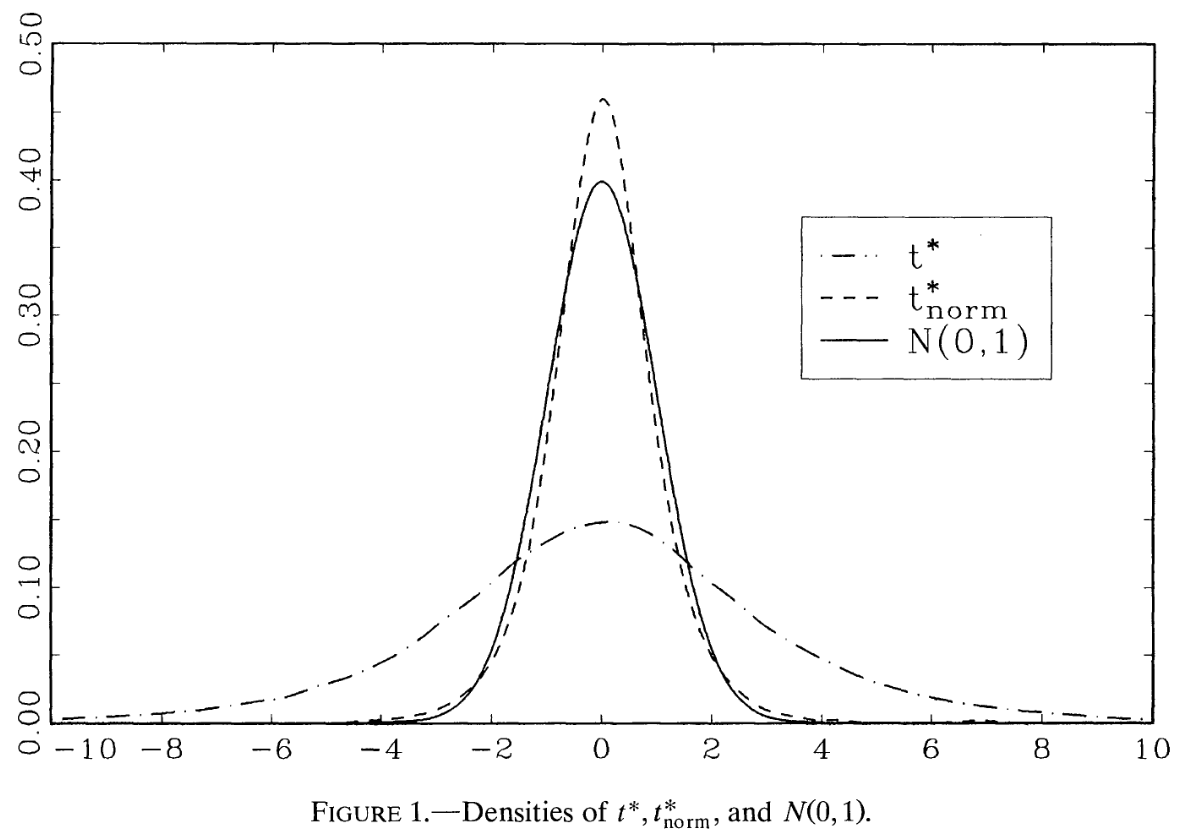
\includegraphics[width=\textwidth]{./Images/KVB.png}

KVB show that in finite samples these tests may outperform tests based on Newey-West standard errors. At a high level, if there is lots of serial correlation KVB is much better, whereas if it is only minor NW is probably fine.  NW suffers when samples are small and serial correlation is large.

KVB, like HAC estimator tests, suffer from serious size distortions (although less so) if the data have highly persistent serial correlation and are close to being non-stationary. KVB also show the finite sample power of their test dominates finite sample power of HAC tests.

\end{document}
